\hsection{Lists}%
\label{sec:lists}%
%
A \pythonilIdx{list} is a mutable sequence of objects which can be accessed via their index~\cite{PSF2024S}.
They work very similar to the strings we already discussed in \cref{sec:str}, but instead of characters, they can contain any kind of objects and they can be modified.%
%
\hsection{Basic Functionality and Examples}%
%
\gitPythonAndOutput{\programmingWithPythonCodeRepo}{02_collections}{lists_1.py}{--args format}{lists:lists_1}{%
A first example for using lists in \python: creating, indexing, printing of and appending elements and other lists to lists.}%
%
\gitPythonAndOutput{\programmingWithPythonCodeRepo}{02_collections}{lists_2.py}{--args format}{lists:lists_2}{%
A second example for using lists in \python: inserting and deleting elemensts, sorting and reversing lists.}%
%
\gitPythonAndOutput{\programmingWithPythonCodeRepo}{02_collections}{lists_3.py}{--args format}{lists:lists_3}{%
A third example for using lists in \python: slicing, adding, and multiplying lists.}%
%
In \cref{lst:lists:lists_1}, we provide some first examples for using lists.
A list can be defined by simply writing its contents, separated by~\pythonilIdx{,} inside square brackets~\pythonilIdx{[...]}.
\pythonil{["apple", "pear", "orange"]} creates a list with three elements, namely the strings \pythonil{"apple"}, \pythonil{"pear"}, and~\pythonil{"orange"}.
If we want to store a list in a variable, then we can use the type hint~\pythonil{list[elementType]}\pythonIdx{list!type hint} where \pythonil{elementType} is to be replaced with the type of the list elements.
\pythonil{fruits: list[str] = ["apple", "pear", "orange"]} therefore creates the list \pythonil{fruits} with the contents listed above.
It also tells any automated type checking tool and other programmers that we intent that only \pythonil{str} values should be stored inside the list.

The length of a list is can be obtained using the \pythonilIdx{len}\pythonIdx{list!len} function.
\pythonil{len(fruits)} will therefore return the value~\pythonil{3}.
We can use lists in \pglspl{fstring} just like any other datatype.
The string representation of \pythonil{fruits} which then would be used is simply \pythonil{"['apple', 'pear', 'orange']"}.%
%
\begin{sloppypar}%
We can add single elements to a list by using the \pythonilIdx{append}\pythonIdx{list!append} method.
Invoking \pythonil{fruits.append("cherry")} will append the string \pythonil{"cherry"} to the list \pythonil{fruits}.
The list then equals \pythonil{["apple", "pear", "orange", "cherry"]} and has \pythonil{len(fruits) == 4}.%
\end{sloppypar}%
%
Of course we can have multiple lists in a program.
In \cref{lst:lists:lists_1}, we now create the second list \pythonil{vegetables} with the three elements \pythonil{"onion"}, \pythonil{"potato"}, and~\pythonil{"leek"}.

An empty list is created with expression~\pythonilIdx{[]}\pythonIdx{empty}, which consists of just the square brackets with no contents inside.
We can append \emph{all} the elements of one collection to a list by using the \pythonilIdx{extend}\pythonIdx{list!extend} method.
We start with the empty list~\pythonil{food} and then invoke~\pythonil{food.extend(fruits)}.
Now all the contents of the list \pythonil{fruits} are appended to \pythonil{food}.
We then invoke~\pythonil{food.extend(vegetables)}, which will add all the elements from the list \pythonil{vegetables} to \pythonil{food} as well.
\pythonil{fruits} and \pythonil{vegetables} remain unchanged during this procedure, but \pythonil{food} now contains all of their elements as well.
It contains all seven fruits and vegetables and its \pythonil{len(food)} is therefore~\pythonil{7}.

We can access the elements of a list by their index, again in the same way we access the characters in a string.
\pythonil{food[0]} returns the first element of the list \pythonil{food}, which is \pythonil{"apple"}.
\pythonil{food[1]} returns the second element of the list \pythonil{food}, which is \pythonil{"pear"}.
And so on.
We can also access the elements using the end of the list as reference:
\pythonil{food[-1]} returns the last element of the list \pythonil{food}, which is \pythonil{"leek"}.
\pythonil{food[-2]} returns the second-to-last element of the list \pythonil{food}, which is \pythonil{"potato"}.
And so on.

Finally, elements can also be deleted from the list by their index.
\pythonil{del food[1]} deletes the second element from the list~\pythonil{food}.
The second element is \pythonil{pear} and if we print \pythonil{food} again, it has indeed disappeared.

In \cref{lst:lists:lists_2}, we illustrate some more operations on lists.
We begin again by creating a list, this time of numbers: \pythonil{numbers: list[int] = [1, 7, 56, 2, 4]} creates (and type-hints) a list of five integers.
If we want to know at which index a certain element in the list is located, we can use the \pythonilIdx{index}\pythonIdx{list!index} method.
\pythonil{numbers.index(7)} will search where the number~\pythonil{7} is located inside~\pythonil{numbers}.
Since it is the second elements and indices start at~0, it returns~\pythonil{1}.
Similarly, \pythonil{numbers.index(7)} returns~\pythonil{3}, because \pythonil{numbers[3] == 2}.

The \pythonilIdx{insert}\pythonIdx{list!insert} method allows us insert an element at a specific index.
The elements which are currently at that or higher indices are moved up one slot.
\pythonil{numbers.insert(2, 12)} will insert the number~\pythonil{12} at index~\pythonil{2} into the list~\pythonil{numbers}.
The element~\pythonil{56} which currently occupies this spot is moved to index~\pythonil{3}, which means that the~\pythonil{2} located at this place is moved to index~\pythonil{4}, which means that the value~\pythonil{4} which right now is stored in this location will move to index~\pythonil{5}.
The list \pythonil{numbers} now looks like this: \pythonil{[1, 7, 12, 56, 2, 4]}.

If we want to remove a specific element from the list without knowing its location, the \pythonilIdx{remove}\pythonIdx{list!remove} method will do the trick.
\pythonil{numbers.remove(56)} searches through the list~\pythonil{numbers} for the element~\pythonil{56} and, once it finds it, deletes it.
The list becomes~\pythonil{[1, 7, 12, 2, 4]}.

We can sort a list inplace by using the~\pythonilIdx{sort}\pythonIdx{list!sort} method.
\pythonil{numbers.sort()} sorts the list~\pythonil{numbers}, which then becomes~\pythonil{[1, 2, 4, 7, 12]}.
Similarly, we can reverse a list, i.e., make the last element become the first, the second-to-last element the second, and so on, by using the method~\pythonil{reverse}\pythonIdx{list!reverse}.
Reversing the list~\pythonil{numbers} after we sorted it will turn it into~\pythonil{[12, 7, 4, 2, 1]}.

If we want to create a list copy of an existing sequence, we can just invoke the constructor~\pythonilIdx{list} directly.
\pythonil{cpy: list[int] = list(numbers)} creates the new list~\pythonil{cpy} which has the same contents as~\pythonil{numbers}.
This means that \pythonil{cpy == numbers} will be~\pythonil{True}, because \pythonil{cpy} is an exact copy of~\pythonil{numbers}.
\pythonil{cpy is numbers}, however, is~\pythonil{False}.
They are not the same object.

We can change~\pythonil{cpy} by deleting its first element via~\pythonil{del cpy[0]}.
\pythonil{numbers} will be unaffected by this and stays unchanged.
Now, both \pythonil{cpy == numbers} and \pythonil{cpy is numbers} will be~\pythonil{False}.

In \cref{lst:lists:lists_3}, we continue our journey through the magical land of \python\ \pythonils{list}.
You can add two lists~\pythonil{a} and~\pythonil{b} using \pythonilIdx{+}\pythonIdx{list!+}, i.e., do \pythonil{c = a + b}.
The result is a new list which contains all elements of the first list~\pythonil{a} followed by all the elements from the second list~\pythonil{b}.
Therefore, the expression \pythonil{[1, 2, 3, 4] + [5, 6, 7]} results in \pythonil{[1, 2, 3, 4, 5, 6, 7]}.
Similarly, if you multiply a list by an integer~\pythonil{n}, you get a new list which equals the old list \pythonil{n}~times concatenated.
\pythonil{[5, 6, 7] * 3}\pythonIdx{*}\pythonIdx{list!*} therefore yields \pythonil{[5, 6, 7, 5, 6, 7, 5, 6, 7]}.

In \cref{sec:strBasicOperations}, we discussed string slicing.
Lists can be sliced in pretty much the same way\pythonIdx{list!slicing}\pythonIdx{slicing}~\cite{PSF2024S}.
When slicing a list~\pythonil{l} or a string, you can provide either two or three values in the square brackets\pythonIdx{[...]}, i.e., either do~\pythonil{l[i:j]} or \pythonil{l[i:j:k]}.
If \pythonil{j < 0}, then it is replaced with~\pythonil{len(l) - j}.
In both the two and three indices case, \pythonil{i} is the inclusive start index and \pythonil{j} is the exclusive end index, i.e., all elements with index~\pythonil{m} such that \pythonil{i <= m < j}.
In other words, the slice will contain elements from~\pythonil{l} whose index is between~\pythonil{i} and~\pythonil{j}, including the element at index~\pythonil{i} but \emph{not} including the element at index~\pythonil{j}.
If a third index~\pythonil{k} is provided, the it is the step length.
\pythonil{l[i:j:k]} selects all items at indices~\pythonil{m} where \pythonil{m = i + n*k}, \pythonil{n >= 0} and \pythonil{i <= m < j}.
If~\pythonil{i} is omitted, i.e., if \pythonil{:j:k} is provided, then \pythonil{i=0} is assumed.
If~\pythonil{j} is omitted, i.e., if \pythonil{i::k} is provided, then \pythonil{j=len(l)} is assumed.

If you have a list \pythonil{l4 = [5, 6, 7, 5, 6, 7, 5, 6, 7]}, then the slice~\pythonil{l4[2:-2]} will return a new list which contains all the elements of~\pythonil{l4} starting from index~\pythonil{2} and up to (excluding) the second-to-last element.
The slice~\pythonil{l4[1::2]} starts at index~\pythonil{1}, continues until the end of the list, and adds every second element.
This results in~\pythonil{[6, 5, 7, 6]}.
As final example, consider the slice~\pythonil{l4[-1:3:-2]}.
It will begin creating the new list at the last element.
The step-length is~\pythonil{-2}, so it will move backwards and add every second element to the new list.
It stops adding elements before reaching index~\pythonil{3}.
Therefore, the result will be the new list~\pythonil{l7 = [7, 5, 6]}.

Notice that the slices we create are independent copies of ranges of the original lists.
The list~\pythonil{l7} is a slice from the list~\pythonil{l4}.
If we modify it, e.g., set \pythonil{l7[1] = 12}, then we set the second element of~\pythonil{l7} to~\pythonil{12}.
\pythonil{l7}~becomes~\pythonil{[7, 12, 6]}.
Now, the second element of~\pythonil{l7} originally is the seventh element of~\pythonil{l4}, namely the \pythonil{5} located at index~\pythonil{6}, which is equivalent to index~\pythonil{-3}.
You may wonder whether this element now also has changed.
It did not.
\pythonil{l4} remains unchanged by any operation on the independent copied slice~\pythonil{l7}.

An interesting functionality is also list unpacking\pythonIdx{list!unpacking}\pythonIdx{unpacking}.
In \cref{sec:strBasicOperations}, the list~\pythonil{l2} contains the three elements~\pythonil{[5, 6, 7]}.
If we know the number of elements in the list in our program, then we can assign them to exactly the same number of variables.
\pythonil{a, b, c = l2} creates and assigns values to three variables \pythonil{a=5}, \pythonil{b=6}, and \pythonil{c=7} by unpacking the list~\pythonil{l2}.%
%
\FloatBarrier%
\endhsection%
%
\hsection{An Example for Errors and a new Tool}%
%
\gitPythonAndOutput{\programmingWithPythonCodeRepo}{02_collections}{lists_error.py}{--args format}{lists:lists_error}{%
A program processing lists which exhibits some subtle errors and inefficiencies.}

Now, in the previous chapter, we learned that static code analysis tools can help us to discover subtle problems in our programs.
Obviously, when dealing with more complex datastructures like lists, there are also more potential problems, more mistakes that one could make.
Let us look at the very short example \cref{lst:lists:lists_error}.
The program consists of only two lines, \pythonil{my_list: list[str] = list([1, 2, 3])} and \pythonil{print(my_list)}.
It does not have any \emph{error} in the strict sense.
We can execute it just fine and it will produce the output \textil{[1, 2, 3]} as shown in \cref{exec:lists:lists_error}.

\gitOutput{\programmingWithPythonCodeRepo}{.}{scripts/mypy.sh 02_collections lists_error.py}{lists:lists_error:mypy}{%
The results of static type checking with \mypy\ of the program given in \cref{lst:lists:lists_error}.}

However, upon closer inspection, we discover some issues.
In a first step, we would apply \mypy~(as~\cref{ut:mypy}) to check for problems with the types of variables.
And indeed, \cref{exec:lists:lists_error:mypy} shows us \emph{three} errors!
We defined \pythonil{my_list} as a list of strings by using the type hint \pythonil{list[str]}.
However, we then set its value to be a list of three integer numbers (hence, three errors).
As promised in the title of this section, we will also use another tool to analyze this program:~\ruff.

\begin{figure}%
\centering%
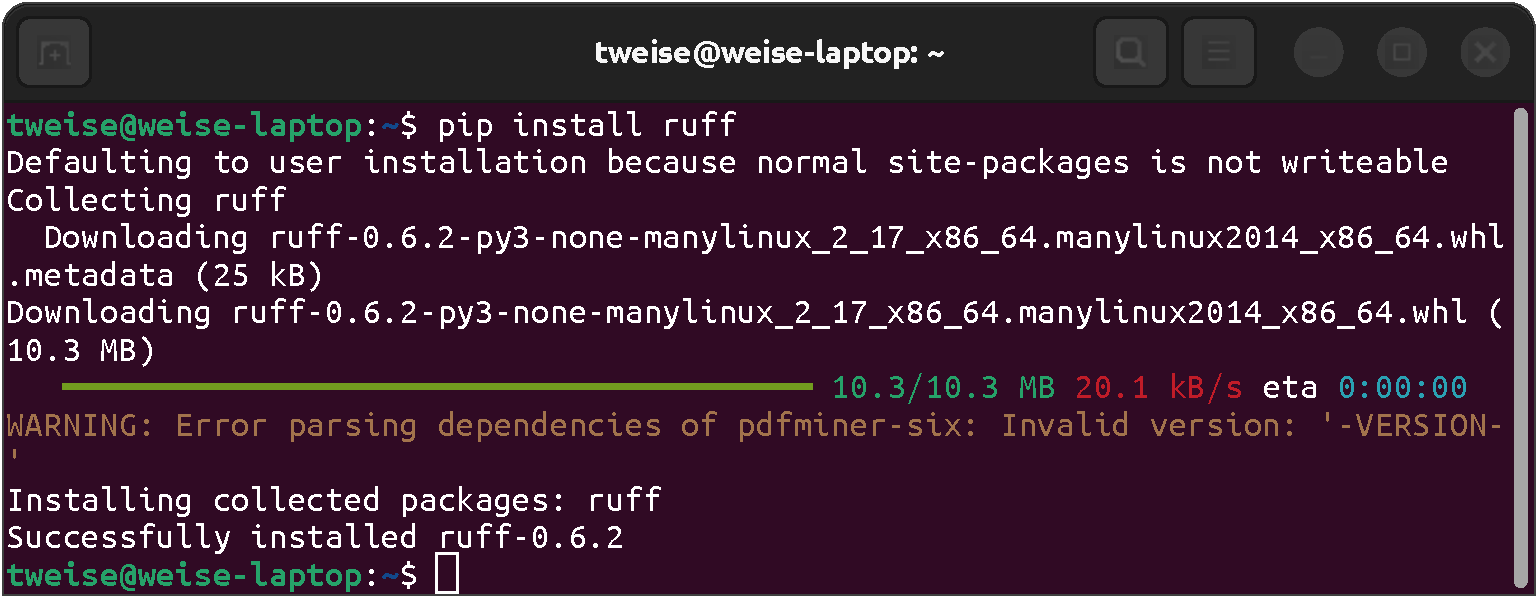
\includegraphics[width=0.7\linewidth]{\currentDir/pipInstallRuff}%
\caption{Installing \ruff\ in a \ubuntu\ \pgls{terminal} via \pip.}%
\label{fig:pipInstallRuff}%
\end{figure}%
%
%
\usefulTool{ruff}{%
\ruff\ is a very fast \python\ \pgls{linter} that checks the code for all kinds of problems, ranging from formatting and style issues over missing documentation to performance problems and potential errors~\cite{M2022RAEFPLACFWIR}. %
It can be installed via \bashil{pip install ruff} as shown in \cref{fig:pipInstallRuff} on \cpageref{fig:pipInstallRuff}. %
You can then apply \ruff\ using the command \bashil{ruff check fileToScan.py}. %
We provide a script for using \ruff\ with a reasonable default configuration in \cref{lst:bash:ruff} on \cpageref{lst:bash:ruff}.%
}%
%
\FloatBarrier%
%
\gitOutput{\programmingWithPythonCodeRepo}{.}{scripts/ruff.sh 02_collections lists_error.py}{lists:lists_error:ruff}{%
The results of linting with \ruff\ of the program given in \cref{lst:lists:lists_error}. (We used the script given in \cref{lst:bash:ruff} on \cpageref{lst:bash:ruff} to apply \ruff.)}%
%
Let us apply \ruff\ to the program \textil{lists_error.py} given in \cref{lst:lists:lists_error}.
\ruff\ finds two errors in this file:
First, it complains that any python file should start with multi-line string specifying the purpose of the file.
The use of such \pglspl{docstring} makes it easier for other programmers to understand what is done by which file in projects that are composed of multiple \python\ scripts.%
%
\bestPractice{module:docstrings}{
Each \python\ file should start with a string describing its purpose~\cite{PEP257}. %
This can either be a single line, like a headline, or a longer text. %
In the second case, the first line must be a headline, followed by an empty line, followed by the rest of the text. %
Either way, it must be a string delimited by~\pythonil{"""..."""}\pythonIdx{"""}~\cite{PEP257,PEP8}.%
\pythonIdx{str!doc}%
}%
%
Additionally, \ruff\ finds that writing \pythonil{list([1, 2, 3])} is actually useless waste of speed and memory:
It basically creates a list via \pythonil{[1, 2, 3]} and then immediately makes a copy of it via the \pythonilIdx{list} function wrapped around the list specification.
We can leave this outer call to \pythonil{list} away.

\gitPythonAndOutput{\programmingWithPythonCodeRepo}{02_collections}{lists_fixed.py}{--args format}{lists:lists_fixed}{%
The corrected version of~\cref{lst:lists:lists_error}, taking into account the information given by \mypy\ in \cref{exec:lists:lists_error:mypy} and \ruff\ in \cref{exec:lists:lists_error:ruff}.}%
%
%
In \cref{lst:lists:lists_fixed} we implement the three recommendations from the two tools.
We change the type hint of the list to \pythonil{list[int]}, which solves the type confusion that \mypy\ discovered.
We remove the useless copying of the list as \ruff\ recommended.
Finally, we add a proper \pgls{docstring} at the top of the file, in which we even document the changes we applied.
The output \cref{exec:lists:lists_fixed} of the new program remains the same.
But now, both tools are satisfied, as shown in \cref{exec:lists:lists_fixed:mypy,exec:lists:lists_fixed:ruff}.
And our program is much clearer and faster.%
%
\FloatBarrier%
%
\gitOutput{\programmingWithPythonCodeRepo}{.}{scripts/mypy.sh 02_collections lists_fixed.py}{lists:lists_fixed:mypy}{%
The results of static type checking with \mypy\ of the program given in \cref{lst:lists:lists_fixed}.}%
%
\gitOutput{\programmingWithPythonCodeRepo}{.}{scripts/ruff.sh 02_collections lists_fixed.py}{lists:lists_fixed:ruff}{%
The results of static type checking with \ruff\ of the program given in \cref{lst:lists:lists_fixed}.}

Well, this was only a two-line program.
But ask yourself:
Did you spot the incorrect type hint when you read the program?
Did you see that we actually created a list and then copied it instead of using it directly?
(The \pgls{docstring} I give you, no chance of seeing that as we did not mention it before.)
Imagine that your job would be to work on a program with thousands of lines that was developed by a colleague.
Wouldn't you love it if that colleague had thoroughly documented and type-hinted and checked their code?
Be that colleague.%
%
\FloatBarrier%
\endhsection%
\endhsection%
%
